% Created by tikzDevice version 0.9 on 2016-01-12 22:38:33
% !TEX encoding = UTF-8 Unicode
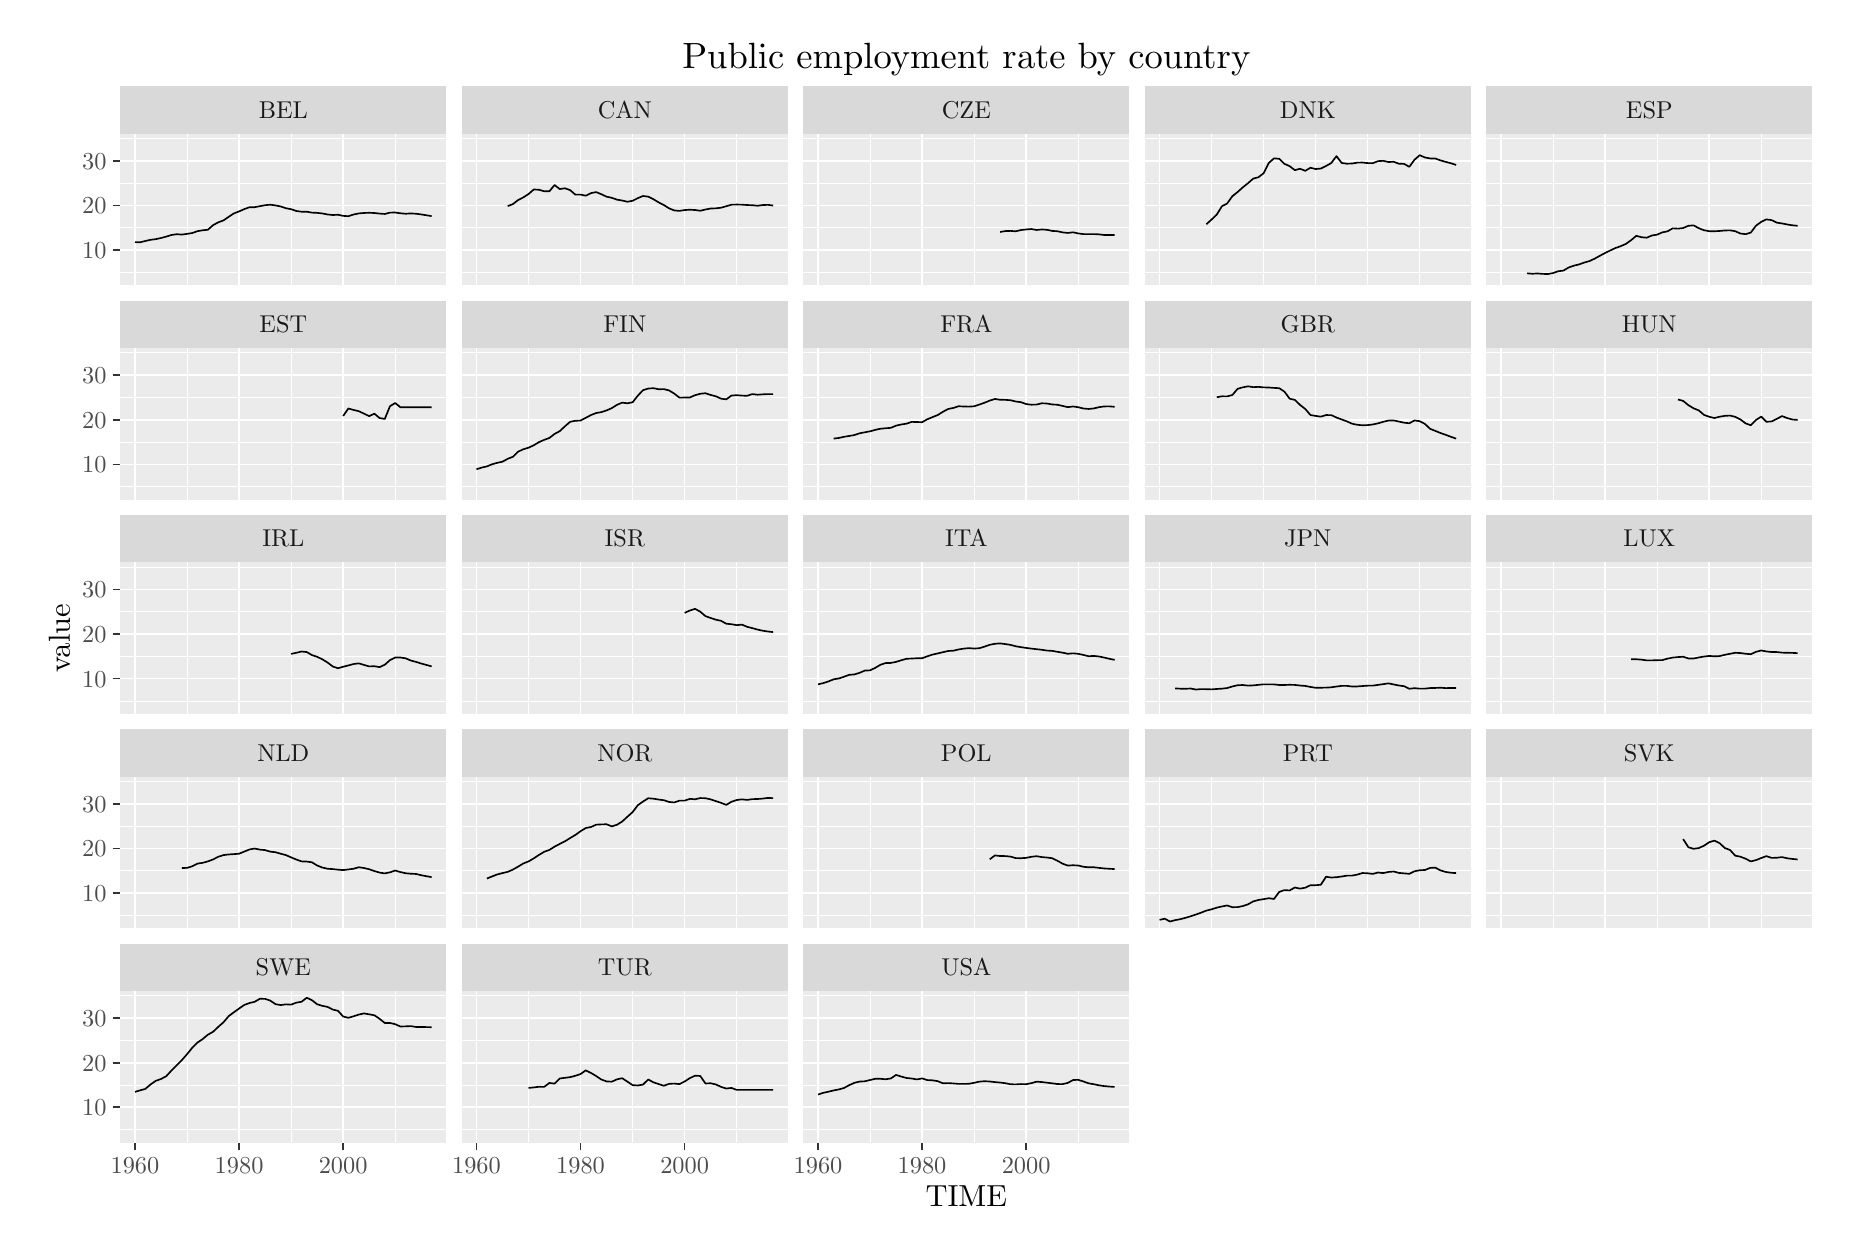
\begin{tikzpicture}[x=1pt,y=1pt]
\definecolor{fillColor}{RGB}{255,255,255}
\path[use as bounding box,fill=fillColor,fill opacity=0.00] (0,0) rectangle (650.43,433.62);
\begin{scope}
\path[clip] (  0.00,  0.00) rectangle (650.43,433.62);
\definecolor{drawColor}{RGB}{255,255,255}
\definecolor{fillColor}{RGB}{255,255,255}

\path[draw=drawColor,line width= 0.6pt,line join=round,line cap=round,fill=fillColor] (  0.00,  0.00) rectangle (650.43,433.62);
\end{scope}
\begin{scope}
\path[clip] ( 33.42,340.48) rectangle (151.33,395.37);
\definecolor{fillColor}{gray}{0.92}

\path[fill=fillColor] ( 33.42,340.48) rectangle (151.33,395.37);
\definecolor{drawColor}{RGB}{255,255,255}

\path[draw=drawColor,line width= 0.3pt,line join=round] ( 33.42,345.22) --
	(151.33,345.22);

\path[draw=drawColor,line width= 0.3pt,line join=round] ( 33.42,361.33) --
	(151.33,361.33);

\path[draw=drawColor,line width= 0.3pt,line join=round] ( 33.42,377.44) --
	(151.33,377.44);

\path[draw=drawColor,line width= 0.3pt,line join=round] ( 33.42,393.55) --
	(151.33,393.55);

\path[draw=drawColor,line width= 0.3pt,line join=round] ( 57.59,340.48) --
	( 57.59,395.37);

\path[draw=drawColor,line width= 0.3pt,line join=round] ( 95.20,340.48) --
	( 95.20,395.37);

\path[draw=drawColor,line width= 0.3pt,line join=round] (132.80,340.48) --
	(132.80,395.37);

\path[draw=drawColor,line width= 0.6pt,line join=round] ( 33.42,353.28) --
	(151.33,353.28);

\path[draw=drawColor,line width= 0.6pt,line join=round] ( 33.42,369.39) --
	(151.33,369.39);

\path[draw=drawColor,line width= 0.6pt,line join=round] ( 33.42,385.50) --
	(151.33,385.50);

\path[draw=drawColor,line width= 0.6pt,line join=round] ( 38.78,340.48) --
	( 38.78,395.37);

\path[draw=drawColor,line width= 0.6pt,line join=round] ( 76.39,340.48) --
	( 76.39,395.37);

\path[draw=drawColor,line width= 0.6pt,line join=round] (114.00,340.48) --
	(114.00,395.37);
\definecolor{drawColor}{RGB}{0,0,0}

\path[draw=drawColor,line width= 0.6pt,line join=round] ( 38.78,356.12) --
	( 40.66,356.07) --
	( 42.54,356.54) --
	( 44.42,356.96) --
	( 46.30,357.20) --
	( 48.19,357.61) --
	( 50.07,358.12) --
	( 51.95,358.70) --
	( 53.83,358.98) --
	( 55.71,358.85) --
	( 57.59,359.11) --
	( 59.47,359.41) --
	( 61.35,360.08) --
	( 63.23,360.40) --
	( 65.11,360.59) --
	( 66.99,362.26) --
	( 68.87,363.28) --
	( 70.75,363.97) --
	( 72.63,365.26) --
	( 74.51,366.51) --
	( 76.39,367.22) --
	( 78.27,368.05) --
	( 80.15,368.73) --
	( 82.03,368.75) --
	( 83.91,369.11) --
	( 85.79,369.47) --
	( 87.67,369.66) --
	( 89.55,369.38) --
	( 91.43,369.00) --
	( 93.31,368.36) --
	( 95.20,368.02) --
	( 97.08,367.37) --
	( 98.96,367.11) --
	(100.84,367.12) --
	(102.72,366.78) --
	(104.60,366.70) --
	(106.48,366.49) --
	(108.36,366.11) --
	(110.24,365.92) --
	(112.12,366.01) --
	(114.00,365.62) --
	(115.88,365.48) --
	(117.76,366.10) --
	(119.64,366.49) --
	(121.52,366.66) --
	(123.40,366.72) --
	(125.28,366.65) --
	(127.16,366.43) --
	(129.04,366.30) --
	(130.92,366.78) --
	(132.80,366.82) --
	(134.68,366.55) --
	(136.56,366.38) --
	(138.44,366.49) --
	(140.32,366.38) --
	(142.21,366.13) --
	(144.09,365.83) --
	(145.97,365.52);
\end{scope}
\begin{scope}
\path[clip] (156.83,340.48) rectangle (274.73,395.37);
\definecolor{fillColor}{gray}{0.92}

\path[fill=fillColor] (156.83,340.48) rectangle (274.73,395.37);
\definecolor{drawColor}{RGB}{255,255,255}

\path[draw=drawColor,line width= 0.3pt,line join=round] (156.83,345.22) --
	(274.73,345.22);

\path[draw=drawColor,line width= 0.3pt,line join=round] (156.83,361.33) --
	(274.73,361.33);

\path[draw=drawColor,line width= 0.3pt,line join=round] (156.83,377.44) --
	(274.73,377.44);

\path[draw=drawColor,line width= 0.3pt,line join=round] (156.83,393.55) --
	(274.73,393.55);

\path[draw=drawColor,line width= 0.3pt,line join=round] (180.99,340.48) --
	(180.99,395.37);

\path[draw=drawColor,line width= 0.3pt,line join=round] (218.60,340.48) --
	(218.60,395.37);

\path[draw=drawColor,line width= 0.3pt,line join=round] (256.20,340.48) --
	(256.20,395.37);

\path[draw=drawColor,line width= 0.6pt,line join=round] (156.83,353.28) --
	(274.73,353.28);

\path[draw=drawColor,line width= 0.6pt,line join=round] (156.83,369.39) --
	(274.73,369.39);

\path[draw=drawColor,line width= 0.6pt,line join=round] (156.83,385.50) --
	(274.73,385.50);

\path[draw=drawColor,line width= 0.6pt,line join=round] (162.18,340.48) --
	(162.18,395.37);

\path[draw=drawColor,line width= 0.6pt,line join=round] (199.79,340.48) --
	(199.79,395.37);

\path[draw=drawColor,line width= 0.6pt,line join=round] (237.40,340.48) --
	(237.40,395.37);
\definecolor{drawColor}{RGB}{0,0,0}

\path[draw=drawColor,line width= 0.6pt,line join=round] (173.47,369.13) --
	(175.35,369.87) --
	(177.23,371.34) --
	(179.11,372.29) --
	(180.99,373.51) --
	(182.87,375.14) --
	(184.75,375.05) --
	(186.63,374.50) --
	(188.51,374.49) --
	(190.39,376.75) --
	(192.27,375.30) --
	(194.15,375.58) --
	(196.03,374.91) --
	(197.91,373.27) --
	(199.79,373.30) --
	(201.67,372.90) --
	(203.55,373.82) --
	(205.43,374.20) --
	(207.31,373.42) --
	(209.19,372.54) --
	(211.07,372.14) --
	(212.96,371.46) --
	(214.84,371.15) --
	(216.72,370.71) --
	(218.60,371.07) --
	(220.48,372.02) --
	(222.36,372.79) --
	(224.24,372.55) --
	(226.12,371.63) --
	(228.00,370.48) --
	(229.88,369.53) --
	(231.76,368.33) --
	(233.64,367.57) --
	(235.52,367.41) --
	(237.40,367.71) --
	(239.28,367.83) --
	(241.16,367.73) --
	(243.04,367.46) --
	(244.92,367.91) --
	(246.80,368.27) --
	(248.68,368.33) --
	(250.56,368.56) --
	(252.44,369.10) --
	(254.32,369.65) --
	(256.20,369.70) --
	(258.08,369.66) --
	(259.97,369.53) --
	(261.85,369.46) --
	(263.73,369.27) --
	(265.61,369.52) --
	(267.49,369.60) --
	(269.37,369.34);
\end{scope}
\begin{scope}
\path[clip] (280.23,340.48) rectangle (398.13,395.37);
\definecolor{fillColor}{gray}{0.92}

\path[fill=fillColor] (280.23,340.48) rectangle (398.13,395.37);
\definecolor{drawColor}{RGB}{255,255,255}

\path[draw=drawColor,line width= 0.3pt,line join=round] (280.23,345.22) --
	(398.13,345.22);

\path[draw=drawColor,line width= 0.3pt,line join=round] (280.23,361.33) --
	(398.13,361.33);

\path[draw=drawColor,line width= 0.3pt,line join=round] (280.23,377.44) --
	(398.13,377.44);

\path[draw=drawColor,line width= 0.3pt,line join=round] (280.23,393.55) --
	(398.13,393.55);

\path[draw=drawColor,line width= 0.3pt,line join=round] (304.39,340.48) --
	(304.39,395.37);

\path[draw=drawColor,line width= 0.3pt,line join=round] (342.00,340.48) --
	(342.00,395.37);

\path[draw=drawColor,line width= 0.3pt,line join=round] (379.61,340.48) --
	(379.61,395.37);

\path[draw=drawColor,line width= 0.6pt,line join=round] (280.23,353.28) --
	(398.13,353.28);

\path[draw=drawColor,line width= 0.6pt,line join=round] (280.23,369.39) --
	(398.13,369.39);

\path[draw=drawColor,line width= 0.6pt,line join=round] (280.23,385.50) --
	(398.13,385.50);

\path[draw=drawColor,line width= 0.6pt,line join=round] (285.59,340.48) --
	(285.59,395.37);

\path[draw=drawColor,line width= 0.6pt,line join=round] (323.19,340.48) --
	(323.19,395.37);

\path[draw=drawColor,line width= 0.6pt,line join=round] (360.80,340.48) --
	(360.80,395.37);
\definecolor{drawColor}{RGB}{0,0,0}

\path[draw=drawColor,line width= 0.6pt,line join=round] (351.40,359.79) --
	(353.28,360.12) --
	(355.16,360.18) --
	(357.04,360.03) --
	(358.92,360.49) --
	(360.80,360.70) --
	(362.68,360.85) --
	(364.56,360.51) --
	(366.44,360.70) --
	(368.32,360.58) --
	(370.20,360.17) --
	(372.08,360.06) --
	(373.96,359.64) --
	(375.84,359.44) --
	(377.73,359.67) --
	(379.61,359.27) --
	(381.49,359.02) --
	(383.37,359.01) --
	(385.25,359.01) --
	(387.13,358.93) --
	(389.01,358.70) --
	(390.89,358.70) --
	(392.77,358.70);
\end{scope}
\begin{scope}
\path[clip] (403.63,340.48) rectangle (521.53,395.37);
\definecolor{fillColor}{gray}{0.92}

\path[fill=fillColor] (403.63,340.48) rectangle (521.53,395.37);
\definecolor{drawColor}{RGB}{255,255,255}

\path[draw=drawColor,line width= 0.3pt,line join=round] (403.63,345.22) --
	(521.53,345.22);

\path[draw=drawColor,line width= 0.3pt,line join=round] (403.63,361.33) --
	(521.53,361.33);

\path[draw=drawColor,line width= 0.3pt,line join=round] (403.63,377.44) --
	(521.53,377.44);

\path[draw=drawColor,line width= 0.3pt,line join=round] (403.63,393.55) --
	(521.53,393.55);

\path[draw=drawColor,line width= 0.3pt,line join=round] (427.79,340.48) --
	(427.79,395.37);

\path[draw=drawColor,line width= 0.3pt,line join=round] (465.40,340.48) --
	(465.40,395.37);

\path[draw=drawColor,line width= 0.3pt,line join=round] (503.01,340.48) --
	(503.01,395.37);

\path[draw=drawColor,line width= 0.6pt,line join=round] (403.63,353.28) --
	(521.53,353.28);

\path[draw=drawColor,line width= 0.6pt,line join=round] (403.63,369.39) --
	(521.53,369.39);

\path[draw=drawColor,line width= 0.6pt,line join=round] (403.63,385.50) --
	(521.53,385.50);

\path[draw=drawColor,line width= 0.6pt,line join=round] (408.99,340.48) --
	(408.99,395.37);

\path[draw=drawColor,line width= 0.6pt,line join=round] (446.59,340.48) --
	(446.59,395.37);

\path[draw=drawColor,line width= 0.6pt,line join=round] (484.20,340.48) --
	(484.20,395.37);
\definecolor{drawColor}{RGB}{0,0,0}

\path[draw=drawColor,line width= 0.6pt,line join=round] (425.91,362.59) --
	(427.79,364.27) --
	(429.67,366.07) --
	(431.55,369.10) --
	(433.43,370.09) --
	(435.31,372.72) --
	(437.19,374.21) --
	(439.07,375.91) --
	(440.95,377.40) --
	(442.83,379.07) --
	(444.71,379.56) --
	(446.59,381.01) --
	(448.48,384.75) --
	(450.36,386.40) --
	(452.24,386.23) --
	(454.12,384.41) --
	(456.00,383.58) --
	(457.88,382.13) --
	(459.76,382.63) --
	(461.64,381.89) --
	(463.52,383.00) --
	(465.40,382.54) --
	(467.28,382.71) --
	(469.16,383.63) --
	(471.04,384.70) --
	(472.92,387.20) --
	(474.80,384.74) --
	(476.68,384.46) --
	(478.56,384.52) --
	(480.44,384.84) --
	(482.32,384.88) --
	(484.20,384.68) --
	(486.08,384.65) --
	(487.96,385.39) --
	(489.84,385.50) --
	(491.72,385.07) --
	(493.60,385.16) --
	(495.49,384.44) --
	(497.37,384.40) --
	(499.25,383.33) --
	(501.13,385.90) --
	(503.01,387.53) --
	(504.89,386.72) --
	(506.77,386.36) --
	(508.65,386.34) --
	(510.53,385.65) --
	(512.41,385.12) --
	(514.29,384.62) --
	(516.17,383.99);
\end{scope}
\begin{scope}
\path[clip] (527.03,340.48) rectangle (644.93,395.37);
\definecolor{fillColor}{gray}{0.92}

\path[fill=fillColor] (527.03,340.48) rectangle (644.93,395.37);
\definecolor{drawColor}{RGB}{255,255,255}

\path[draw=drawColor,line width= 0.3pt,line join=round] (527.03,345.22) --
	(644.93,345.22);

\path[draw=drawColor,line width= 0.3pt,line join=round] (527.03,361.33) --
	(644.93,361.33);

\path[draw=drawColor,line width= 0.3pt,line join=round] (527.03,377.44) --
	(644.93,377.44);

\path[draw=drawColor,line width= 0.3pt,line join=round] (527.03,393.55) --
	(644.93,393.55);

\path[draw=drawColor,line width= 0.3pt,line join=round] (551.19,340.48) --
	(551.19,395.37);

\path[draw=drawColor,line width= 0.3pt,line join=round] (588.80,340.48) --
	(588.80,395.37);

\path[draw=drawColor,line width= 0.3pt,line join=round] (626.41,340.48) --
	(626.41,395.37);

\path[draw=drawColor,line width= 0.6pt,line join=round] (527.03,353.28) --
	(644.93,353.28);

\path[draw=drawColor,line width= 0.6pt,line join=round] (527.03,369.39) --
	(644.93,369.39);

\path[draw=drawColor,line width= 0.6pt,line join=round] (527.03,385.50) --
	(644.93,385.50);

\path[draw=drawColor,line width= 0.6pt,line join=round] (532.39,340.48) --
	(532.39,395.37);

\path[draw=drawColor,line width= 0.6pt,line join=round] (570.00,340.48) --
	(570.00,395.37);

\path[draw=drawColor,line width= 0.6pt,line join=round] (607.60,340.48) --
	(607.60,395.37);
\definecolor{drawColor}{RGB}{0,0,0}

\path[draw=drawColor,line width= 0.6pt,line join=round] (541.79,344.85) --
	(543.67,344.70) --
	(545.55,344.80) --
	(547.43,344.66) --
	(549.31,344.58) --
	(551.19,344.95) --
	(553.07,345.60) --
	(554.95,345.84) --
	(556.83,346.96) --
	(558.71,347.62) --
	(560.59,348.07) --
	(562.47,348.75) --
	(564.35,349.27) --
	(566.24,350.16) --
	(568.12,351.19) --
	(570.00,352.20) --
	(571.88,353.13) --
	(573.76,353.99) --
	(575.64,354.66) --
	(577.52,355.48) --
	(579.40,356.84) --
	(581.28,358.40) --
	(583.16,357.89) --
	(585.04,357.72) --
	(586.92,358.53) --
	(588.80,358.83) --
	(590.68,359.65) --
	(592.56,360.03) --
	(594.44,361.11) --
	(596.32,360.99) --
	(598.20,361.22) --
	(600.08,362.02) --
	(601.96,362.19) --
	(603.84,361.16) --
	(605.72,360.42) --
	(607.60,360.08) --
	(609.48,360.05) --
	(611.36,360.15) --
	(613.25,360.33) --
	(615.13,360.38) --
	(617.01,360.08) --
	(618.89,359.23) --
	(620.77,359.00) --
	(622.65,359.57) --
	(624.53,362.08) --
	(626.41,363.43) --
	(628.29,364.35) --
	(630.17,364.07) --
	(632.05,363.16) --
	(633.93,362.87) --
	(635.81,362.50) --
	(637.69,362.21) --
	(639.57,362.01);
\end{scope}
\begin{scope}
\path[clip] ( 33.42,263.03) rectangle (151.33,317.92);
\definecolor{fillColor}{gray}{0.92}

\path[fill=fillColor] ( 33.42,263.03) rectangle (151.33,317.92);
\definecolor{drawColor}{RGB}{255,255,255}

\path[draw=drawColor,line width= 0.3pt,line join=round] ( 33.42,267.78) --
	(151.33,267.78);

\path[draw=drawColor,line width= 0.3pt,line join=round] ( 33.42,283.88) --
	(151.33,283.88);

\path[draw=drawColor,line width= 0.3pt,line join=round] ( 33.42,299.99) --
	(151.33,299.99);

\path[draw=drawColor,line width= 0.3pt,line join=round] ( 33.42,316.10) --
	(151.33,316.10);

\path[draw=drawColor,line width= 0.3pt,line join=round] ( 57.59,263.03) --
	( 57.59,317.92);

\path[draw=drawColor,line width= 0.3pt,line join=round] ( 95.20,263.03) --
	( 95.20,317.92);

\path[draw=drawColor,line width= 0.3pt,line join=round] (132.80,263.03) --
	(132.80,317.92);

\path[draw=drawColor,line width= 0.6pt,line join=round] ( 33.42,275.83) --
	(151.33,275.83);

\path[draw=drawColor,line width= 0.6pt,line join=round] ( 33.42,291.94) --
	(151.33,291.94);

\path[draw=drawColor,line width= 0.6pt,line join=round] ( 33.42,308.05) --
	(151.33,308.05);

\path[draw=drawColor,line width= 0.6pt,line join=round] ( 38.78,263.03) --
	( 38.78,317.92);

\path[draw=drawColor,line width= 0.6pt,line join=round] ( 76.39,263.03) --
	( 76.39,317.92);

\path[draw=drawColor,line width= 0.6pt,line join=round] (114.00,263.03) --
	(114.00,317.92);
\definecolor{drawColor}{RGB}{0,0,0}

\path[draw=drawColor,line width= 0.6pt,line join=round] (114.00,293.30) --
	(115.88,296.01) --
	(117.76,295.48) --
	(119.64,295.03) --
	(121.52,294.16) --
	(123.40,293.25) --
	(125.28,294.13) --
	(127.16,292.56) --
	(129.04,292.23) --
	(130.92,296.84) --
	(132.80,297.98) --
	(134.68,296.46) --
	(136.56,296.46) --
	(138.44,296.46) --
	(140.32,296.46) --
	(142.21,296.46) --
	(144.09,296.46) --
	(145.97,296.46);
\end{scope}
\begin{scope}
\path[clip] (156.83,263.03) rectangle (274.73,317.92);
\definecolor{fillColor}{gray}{0.92}

\path[fill=fillColor] (156.83,263.03) rectangle (274.73,317.92);
\definecolor{drawColor}{RGB}{255,255,255}

\path[draw=drawColor,line width= 0.3pt,line join=round] (156.83,267.78) --
	(274.73,267.78);

\path[draw=drawColor,line width= 0.3pt,line join=round] (156.83,283.88) --
	(274.73,283.88);

\path[draw=drawColor,line width= 0.3pt,line join=round] (156.83,299.99) --
	(274.73,299.99);

\path[draw=drawColor,line width= 0.3pt,line join=round] (156.83,316.10) --
	(274.73,316.10);

\path[draw=drawColor,line width= 0.3pt,line join=round] (180.99,263.03) --
	(180.99,317.92);

\path[draw=drawColor,line width= 0.3pt,line join=round] (218.60,263.03) --
	(218.60,317.92);

\path[draw=drawColor,line width= 0.3pt,line join=round] (256.20,263.03) --
	(256.20,317.92);

\path[draw=drawColor,line width= 0.6pt,line join=round] (156.83,275.83) --
	(274.73,275.83);

\path[draw=drawColor,line width= 0.6pt,line join=round] (156.83,291.94) --
	(274.73,291.94);

\path[draw=drawColor,line width= 0.6pt,line join=round] (156.83,308.05) --
	(274.73,308.05);

\path[draw=drawColor,line width= 0.6pt,line join=round] (162.18,263.03) --
	(162.18,317.92);

\path[draw=drawColor,line width= 0.6pt,line join=round] (199.79,263.03) --
	(199.79,317.92);

\path[draw=drawColor,line width= 0.6pt,line join=round] (237.40,263.03) --
	(237.40,317.92);
\definecolor{drawColor}{RGB}{0,0,0}

\path[draw=drawColor,line width= 0.6pt,line join=round] (162.18,274.04) --
	(164.06,274.66) --
	(165.95,275.08) --
	(167.83,275.86) --
	(169.71,276.38) --
	(171.59,276.79) --
	(173.47,277.83) --
	(175.35,278.57) --
	(177.23,280.40) --
	(179.11,281.28) --
	(180.99,281.84) --
	(182.87,282.72) --
	(184.75,283.84) --
	(186.63,284.67) --
	(188.51,285.36) --
	(190.39,286.81) --
	(192.27,287.83) --
	(194.15,289.58) --
	(196.03,291.21) --
	(197.91,291.57) --
	(199.79,291.65) --
	(201.67,292.64) --
	(203.55,293.64) --
	(205.43,294.37) --
	(207.31,294.70) --
	(209.19,295.32) --
	(211.07,296.13) --
	(212.96,297.34) --
	(214.84,298.13) --
	(216.72,297.88) --
	(218.60,298.26) --
	(220.48,300.65) --
	(222.36,302.63) --
	(224.24,303.21) --
	(226.12,303.35) --
	(228.00,302.96) --
	(229.88,303.01) --
	(231.76,302.54) --
	(233.64,301.39) --
	(235.52,299.93) --
	(237.40,299.96) --
	(239.28,299.98) --
	(241.16,300.82) --
	(243.04,301.33) --
	(244.92,301.53) --
	(246.80,300.90) --
	(248.68,300.41) --
	(250.56,299.56) --
	(252.44,299.31) --
	(254.32,300.69) --
	(256.20,300.81) --
	(258.08,300.67) --
	(259.97,300.59) --
	(261.85,301.21) --
	(263.73,300.99) --
	(265.61,301.12) --
	(267.49,301.21) --
	(269.37,301.21);
\end{scope}
\begin{scope}
\path[clip] (280.23,263.03) rectangle (398.13,317.92);
\definecolor{fillColor}{gray}{0.92}

\path[fill=fillColor] (280.23,263.03) rectangle (398.13,317.92);
\definecolor{drawColor}{RGB}{255,255,255}

\path[draw=drawColor,line width= 0.3pt,line join=round] (280.23,267.78) --
	(398.13,267.78);

\path[draw=drawColor,line width= 0.3pt,line join=round] (280.23,283.88) --
	(398.13,283.88);

\path[draw=drawColor,line width= 0.3pt,line join=round] (280.23,299.99) --
	(398.13,299.99);

\path[draw=drawColor,line width= 0.3pt,line join=round] (280.23,316.10) --
	(398.13,316.10);

\path[draw=drawColor,line width= 0.3pt,line join=round] (304.39,263.03) --
	(304.39,317.92);

\path[draw=drawColor,line width= 0.3pt,line join=round] (342.00,263.03) --
	(342.00,317.92);

\path[draw=drawColor,line width= 0.3pt,line join=round] (379.61,263.03) --
	(379.61,317.92);

\path[draw=drawColor,line width= 0.6pt,line join=round] (280.23,275.83) --
	(398.13,275.83);

\path[draw=drawColor,line width= 0.6pt,line join=round] (280.23,291.94) --
	(398.13,291.94);

\path[draw=drawColor,line width= 0.6pt,line join=round] (280.23,308.05) --
	(398.13,308.05);

\path[draw=drawColor,line width= 0.6pt,line join=round] (285.59,263.03) --
	(285.59,317.92);

\path[draw=drawColor,line width= 0.6pt,line join=round] (323.19,263.03) --
	(323.19,317.92);

\path[draw=drawColor,line width= 0.6pt,line join=round] (360.80,263.03) --
	(360.80,317.92);
\definecolor{drawColor}{RGB}{0,0,0}

\path[draw=drawColor,line width= 0.6pt,line join=round] (291.23,285.13) --
	(293.11,285.36) --
	(294.99,285.78) --
	(296.87,286.08) --
	(298.75,286.41) --
	(300.63,287.04) --
	(302.51,287.41) --
	(304.39,287.76) --
	(306.27,288.28) --
	(308.15,288.70) --
	(310.03,288.86) --
	(311.91,289.02) --
	(313.79,289.81) --
	(315.67,290.23) --
	(317.55,290.52) --
	(319.43,291.17) --
	(321.31,291.12) --
	(323.19,291.05) --
	(325.07,292.11) --
	(326.95,292.88) --
	(328.83,293.63) --
	(330.72,294.82) --
	(332.60,295.83) --
	(334.48,296.20) --
	(336.36,296.82) --
	(338.24,296.73) --
	(340.12,296.68) --
	(342.00,296.80) --
	(343.88,297.42) --
	(345.76,298.09) --
	(347.64,298.86) --
	(349.52,299.45) --
	(351.40,299.16) --
	(353.28,299.13) --
	(355.16,298.99) --
	(357.04,298.53) --
	(358.92,298.29) --
	(360.80,297.60) --
	(362.68,297.38) --
	(364.56,297.42) --
	(366.44,297.89) --
	(368.32,297.81) --
	(370.20,297.46) --
	(372.08,297.36) --
	(373.96,296.94) --
	(375.84,296.49) --
	(377.73,296.73) --
	(379.61,296.47) --
	(381.49,296.00) --
	(383.37,295.84) --
	(385.25,296.02) --
	(387.13,296.49) --
	(389.01,296.75) --
	(390.89,296.77) --
	(392.77,296.62);
\end{scope}
\begin{scope}
\path[clip] (403.63,263.03) rectangle (521.53,317.92);
\definecolor{fillColor}{gray}{0.92}

\path[fill=fillColor] (403.63,263.03) rectangle (521.53,317.92);
\definecolor{drawColor}{RGB}{255,255,255}

\path[draw=drawColor,line width= 0.3pt,line join=round] (403.63,267.78) --
	(521.53,267.78);

\path[draw=drawColor,line width= 0.3pt,line join=round] (403.63,283.88) --
	(521.53,283.88);

\path[draw=drawColor,line width= 0.3pt,line join=round] (403.63,299.99) --
	(521.53,299.99);

\path[draw=drawColor,line width= 0.3pt,line join=round] (403.63,316.10) --
	(521.53,316.10);

\path[draw=drawColor,line width= 0.3pt,line join=round] (427.79,263.03) --
	(427.79,317.92);

\path[draw=drawColor,line width= 0.3pt,line join=round] (465.40,263.03) --
	(465.40,317.92);

\path[draw=drawColor,line width= 0.3pt,line join=round] (503.01,263.03) --
	(503.01,317.92);

\path[draw=drawColor,line width= 0.6pt,line join=round] (403.63,275.83) --
	(521.53,275.83);

\path[draw=drawColor,line width= 0.6pt,line join=round] (403.63,291.94) --
	(521.53,291.94);

\path[draw=drawColor,line width= 0.6pt,line join=round] (403.63,308.05) --
	(521.53,308.05);

\path[draw=drawColor,line width= 0.6pt,line join=round] (408.99,263.03) --
	(408.99,317.92);

\path[draw=drawColor,line width= 0.6pt,line join=round] (446.59,263.03) --
	(446.59,317.92);

\path[draw=drawColor,line width= 0.6pt,line join=round] (484.20,263.03) --
	(484.20,317.92);
\definecolor{drawColor}{RGB}{0,0,0}

\path[draw=drawColor,line width= 0.6pt,line join=round] (429.67,300.06) --
	(431.55,300.41) --
	(433.43,300.38) --
	(435.31,300.88) --
	(437.19,303.11) --
	(439.07,303.65) --
	(440.95,304.02) --
	(442.83,303.72) --
	(444.71,303.82) --
	(446.59,303.64) --
	(448.48,303.59) --
	(450.36,303.45) --
	(452.24,303.34) --
	(454.12,302.10) --
	(456.00,299.56) --
	(457.88,299.11) --
	(459.76,297.30) --
	(461.64,295.85) --
	(463.52,293.65) --
	(465.40,293.32) --
	(467.28,293.06) --
	(469.16,293.63) --
	(471.04,293.62) --
	(472.92,292.75) --
	(474.80,292.04) --
	(476.68,291.36) --
	(478.56,290.51) --
	(480.44,290.12) --
	(482.32,289.94) --
	(484.20,290.01) --
	(486.08,290.23) --
	(487.96,290.65) --
	(489.84,291.20) --
	(491.72,291.64) --
	(493.60,291.69) --
	(495.49,291.29) --
	(497.37,290.87) --
	(499.25,290.68) --
	(501.13,291.69) --
	(503.01,291.41) --
	(504.89,290.43) --
	(506.77,288.65) --
	(508.65,287.91) --
	(510.53,287.14) --
	(512.41,286.48) --
	(514.29,285.78) --
	(516.17,285.11);
\end{scope}
\begin{scope}
\path[clip] (527.03,263.03) rectangle (644.93,317.92);
\definecolor{fillColor}{gray}{0.92}

\path[fill=fillColor] (527.03,263.03) rectangle (644.93,317.92);
\definecolor{drawColor}{RGB}{255,255,255}

\path[draw=drawColor,line width= 0.3pt,line join=round] (527.03,267.78) --
	(644.93,267.78);

\path[draw=drawColor,line width= 0.3pt,line join=round] (527.03,283.88) --
	(644.93,283.88);

\path[draw=drawColor,line width= 0.3pt,line join=round] (527.03,299.99) --
	(644.93,299.99);

\path[draw=drawColor,line width= 0.3pt,line join=round] (527.03,316.10) --
	(644.93,316.10);

\path[draw=drawColor,line width= 0.3pt,line join=round] (551.19,263.03) --
	(551.19,317.92);

\path[draw=drawColor,line width= 0.3pt,line join=round] (588.80,263.03) --
	(588.80,317.92);

\path[draw=drawColor,line width= 0.3pt,line join=round] (626.41,263.03) --
	(626.41,317.92);

\path[draw=drawColor,line width= 0.6pt,line join=round] (527.03,275.83) --
	(644.93,275.83);

\path[draw=drawColor,line width= 0.6pt,line join=round] (527.03,291.94) --
	(644.93,291.94);

\path[draw=drawColor,line width= 0.6pt,line join=round] (527.03,308.05) --
	(644.93,308.05);

\path[draw=drawColor,line width= 0.6pt,line join=round] (532.39,263.03) --
	(532.39,317.92);

\path[draw=drawColor,line width= 0.6pt,line join=round] (570.00,263.03) --
	(570.00,317.92);

\path[draw=drawColor,line width= 0.6pt,line join=round] (607.60,263.03) --
	(607.60,317.92);
\definecolor{drawColor}{RGB}{0,0,0}

\path[draw=drawColor,line width= 0.6pt,line join=round] (596.32,299.26) --
	(598.20,298.75) --
	(600.08,297.21) --
	(601.96,296.07) --
	(603.84,295.32) --
	(605.72,293.70) --
	(607.60,293.02) --
	(609.48,292.56) --
	(611.36,293.03) --
	(613.25,293.35) --
	(615.13,293.45) --
	(617.01,293.00) --
	(618.89,292.05) --
	(620.77,290.63) --
	(622.65,289.95) --
	(624.53,291.87) --
	(626.41,293.07) --
	(628.29,291.20) --
	(630.17,291.34) --
	(632.05,292.25) --
	(633.93,293.27) --
	(635.81,292.53) --
	(637.69,292.02) --
	(639.57,291.87);
\end{scope}
\begin{scope}
\path[clip] ( 33.42,185.58) rectangle (151.33,240.47);
\definecolor{fillColor}{gray}{0.92}

\path[fill=fillColor] ( 33.42,185.58) rectangle (151.33,240.47);
\definecolor{drawColor}{RGB}{255,255,255}

\path[draw=drawColor,line width= 0.3pt,line join=round] ( 33.42,190.33) --
	(151.33,190.33);

\path[draw=drawColor,line width= 0.3pt,line join=round] ( 33.42,206.44) --
	(151.33,206.44);

\path[draw=drawColor,line width= 0.3pt,line join=round] ( 33.42,222.55) --
	(151.33,222.55);

\path[draw=drawColor,line width= 0.3pt,line join=round] ( 33.42,238.65) --
	(151.33,238.65);

\path[draw=drawColor,line width= 0.3pt,line join=round] ( 57.59,185.58) --
	( 57.59,240.47);

\path[draw=drawColor,line width= 0.3pt,line join=round] ( 95.20,185.58) --
	( 95.20,240.47);

\path[draw=drawColor,line width= 0.3pt,line join=round] (132.80,185.58) --
	(132.80,240.47);

\path[draw=drawColor,line width= 0.6pt,line join=round] ( 33.42,198.38) --
	(151.33,198.38);

\path[draw=drawColor,line width= 0.6pt,line join=round] ( 33.42,214.49) --
	(151.33,214.49);

\path[draw=drawColor,line width= 0.6pt,line join=round] ( 33.42,230.60) --
	(151.33,230.60);

\path[draw=drawColor,line width= 0.6pt,line join=round] ( 38.78,185.58) --
	( 38.78,240.47);

\path[draw=drawColor,line width= 0.6pt,line join=round] ( 76.39,185.58) --
	( 76.39,240.47);

\path[draw=drawColor,line width= 0.6pt,line join=round] (114.00,185.58) --
	(114.00,240.47);
\definecolor{drawColor}{RGB}{0,0,0}

\path[draw=drawColor,line width= 0.6pt,line join=round] ( 95.20,207.32) --
	( 97.08,207.74) --
	( 98.96,208.19) --
	(100.84,208.00) --
	(102.72,206.90) --
	(104.60,206.28) --
	(106.48,205.37) --
	(108.36,204.22) --
	(110.24,202.79) --
	(112.12,202.15) --
	(114.00,202.69) --
	(115.88,203.16) --
	(117.76,203.67) --
	(119.64,203.92) --
	(121.52,203.35) --
	(123.40,202.81) --
	(125.28,202.88) --
	(127.16,202.55) --
	(129.04,203.42) --
	(130.92,205.09) --
	(132.80,206.02) --
	(134.68,206.02) --
	(136.56,205.74) --
	(138.44,204.94) --
	(140.32,204.44) --
	(142.21,203.85) --
	(144.09,203.34) --
	(145.97,202.81);
\end{scope}
\begin{scope}
\path[clip] (156.83,185.58) rectangle (274.73,240.47);
\definecolor{fillColor}{gray}{0.92}

\path[fill=fillColor] (156.83,185.58) rectangle (274.73,240.47);
\definecolor{drawColor}{RGB}{255,255,255}

\path[draw=drawColor,line width= 0.3pt,line join=round] (156.83,190.33) --
	(274.73,190.33);

\path[draw=drawColor,line width= 0.3pt,line join=round] (156.83,206.44) --
	(274.73,206.44);

\path[draw=drawColor,line width= 0.3pt,line join=round] (156.83,222.55) --
	(274.73,222.55);

\path[draw=drawColor,line width= 0.3pt,line join=round] (156.83,238.65) --
	(274.73,238.65);

\path[draw=drawColor,line width= 0.3pt,line join=round] (180.99,185.58) --
	(180.99,240.47);

\path[draw=drawColor,line width= 0.3pt,line join=round] (218.60,185.58) --
	(218.60,240.47);

\path[draw=drawColor,line width= 0.3pt,line join=round] (256.20,185.58) --
	(256.20,240.47);

\path[draw=drawColor,line width= 0.6pt,line join=round] (156.83,198.38) --
	(274.73,198.38);

\path[draw=drawColor,line width= 0.6pt,line join=round] (156.83,214.49) --
	(274.73,214.49);

\path[draw=drawColor,line width= 0.6pt,line join=round] (156.83,230.60) --
	(274.73,230.60);

\path[draw=drawColor,line width= 0.6pt,line join=round] (162.18,185.58) --
	(162.18,240.47);

\path[draw=drawColor,line width= 0.6pt,line join=round] (199.79,185.58) --
	(199.79,240.47);

\path[draw=drawColor,line width= 0.6pt,line join=round] (237.40,185.58) --
	(237.40,240.47);
\definecolor{drawColor}{RGB}{0,0,0}

\path[draw=drawColor,line width= 0.6pt,line join=round] (237.40,222.16) --
	(239.28,223.01) --
	(241.16,223.61) --
	(243.04,222.58) --
	(244.92,220.97) --
	(246.80,220.31) --
	(248.68,219.69) --
	(250.56,219.28) --
	(252.44,218.23) --
	(254.32,218.06) --
	(256.20,217.71) --
	(258.08,217.92) --
	(259.97,217.12) --
	(261.85,216.65) --
	(263.73,216.12) --
	(265.61,215.71) --
	(267.49,215.42) --
	(269.37,215.20);
\end{scope}
\begin{scope}
\path[clip] (280.23,185.58) rectangle (398.13,240.47);
\definecolor{fillColor}{gray}{0.92}

\path[fill=fillColor] (280.23,185.58) rectangle (398.13,240.47);
\definecolor{drawColor}{RGB}{255,255,255}

\path[draw=drawColor,line width= 0.3pt,line join=round] (280.23,190.33) --
	(398.13,190.33);

\path[draw=drawColor,line width= 0.3pt,line join=round] (280.23,206.44) --
	(398.13,206.44);

\path[draw=drawColor,line width= 0.3pt,line join=round] (280.23,222.55) --
	(398.13,222.55);

\path[draw=drawColor,line width= 0.3pt,line join=round] (280.23,238.65) --
	(398.13,238.65);

\path[draw=drawColor,line width= 0.3pt,line join=round] (304.39,185.58) --
	(304.39,240.47);

\path[draw=drawColor,line width= 0.3pt,line join=round] (342.00,185.58) --
	(342.00,240.47);

\path[draw=drawColor,line width= 0.3pt,line join=round] (379.61,185.58) --
	(379.61,240.47);

\path[draw=drawColor,line width= 0.6pt,line join=round] (280.23,198.38) --
	(398.13,198.38);

\path[draw=drawColor,line width= 0.6pt,line join=round] (280.23,214.49) --
	(398.13,214.49);

\path[draw=drawColor,line width= 0.6pt,line join=round] (280.23,230.60) --
	(398.13,230.60);

\path[draw=drawColor,line width= 0.6pt,line join=round] (285.59,185.58) --
	(285.59,240.47);

\path[draw=drawColor,line width= 0.6pt,line join=round] (323.19,185.58) --
	(323.19,240.47);

\path[draw=drawColor,line width= 0.6pt,line join=round] (360.80,185.58) --
	(360.80,240.47);
\definecolor{drawColor}{RGB}{0,0,0}

\path[draw=drawColor,line width= 0.6pt,line join=round] (285.59,196.33) --
	(287.47,196.77) --
	(289.35,197.38) --
	(291.23,198.15) --
	(293.11,198.46) --
	(294.99,199.09) --
	(296.87,199.77) --
	(298.75,199.91) --
	(300.63,200.51) --
	(302.51,201.30) --
	(304.39,201.39) --
	(306.27,202.29) --
	(308.15,203.41) --
	(310.03,204.02) --
	(311.91,204.07) --
	(313.79,204.44) --
	(315.67,205.03) --
	(317.55,205.57) --
	(319.43,205.65) --
	(321.31,205.76) --
	(323.19,205.75) --
	(325.07,206.47) --
	(326.95,207.07) --
	(328.83,207.50) --
	(330.72,207.94) --
	(332.60,208.38) --
	(334.48,208.49) --
	(336.36,208.93) --
	(338.24,209.24) --
	(340.12,209.41) --
	(342.00,209.27) --
	(343.88,209.38) --
	(345.76,209.96) --
	(347.64,210.62) --
	(349.52,210.99) --
	(351.40,211.12) --
	(353.28,210.88) --
	(355.16,210.58) --
	(357.04,210.08) --
	(358.92,209.77) --
	(360.80,209.49) --
	(362.68,209.24) --
	(364.56,209.03) --
	(366.44,208.82) --
	(368.32,208.53) --
	(370.20,208.42) --
	(372.08,208.09) --
	(373.96,207.78) --
	(375.84,207.37) --
	(377.73,207.53) --
	(379.61,207.37) --
	(381.49,206.95) --
	(383.37,206.49) --
	(385.25,206.60) --
	(387.13,206.39) --
	(389.01,206.00) --
	(390.89,205.55) --
	(392.77,205.18);
\end{scope}
\begin{scope}
\path[clip] (403.63,185.58) rectangle (521.53,240.47);
\definecolor{fillColor}{gray}{0.92}

\path[fill=fillColor] (403.63,185.58) rectangle (521.53,240.47);
\definecolor{drawColor}{RGB}{255,255,255}

\path[draw=drawColor,line width= 0.3pt,line join=round] (403.63,190.33) --
	(521.53,190.33);

\path[draw=drawColor,line width= 0.3pt,line join=round] (403.63,206.44) --
	(521.53,206.44);

\path[draw=drawColor,line width= 0.3pt,line join=round] (403.63,222.55) --
	(521.53,222.55);

\path[draw=drawColor,line width= 0.3pt,line join=round] (403.63,238.65) --
	(521.53,238.65);

\path[draw=drawColor,line width= 0.3pt,line join=round] (427.79,185.58) --
	(427.79,240.47);

\path[draw=drawColor,line width= 0.3pt,line join=round] (465.40,185.58) --
	(465.40,240.47);

\path[draw=drawColor,line width= 0.3pt,line join=round] (503.01,185.58) --
	(503.01,240.47);

\path[draw=drawColor,line width= 0.6pt,line join=round] (403.63,198.38) --
	(521.53,198.38);

\path[draw=drawColor,line width= 0.6pt,line join=round] (403.63,214.49) --
	(521.53,214.49);

\path[draw=drawColor,line width= 0.6pt,line join=round] (403.63,230.60) --
	(521.53,230.60);

\path[draw=drawColor,line width= 0.6pt,line join=round] (408.99,185.58) --
	(408.99,240.47);

\path[draw=drawColor,line width= 0.6pt,line join=round] (446.59,185.58) --
	(446.59,240.47);

\path[draw=drawColor,line width= 0.6pt,line join=round] (484.20,185.58) --
	(484.20,240.47);
\definecolor{drawColor}{RGB}{0,0,0}

\path[draw=drawColor,line width= 0.6pt,line join=round] (414.63,194.86) --
	(416.51,194.76) --
	(418.39,194.74) --
	(420.27,194.82) --
	(422.15,194.45) --
	(424.03,194.61) --
	(425.91,194.58) --
	(427.79,194.51) --
	(429.67,194.66) --
	(431.55,194.77) --
	(433.43,194.99) --
	(435.31,195.56) --
	(437.19,196.00) --
	(439.07,196.09) --
	(440.95,195.87) --
	(442.83,195.95) --
	(444.71,196.15) --
	(446.59,196.33) --
	(448.48,196.33) --
	(450.36,196.30) --
	(452.24,196.10) --
	(454.12,196.10) --
	(456.00,196.17) --
	(457.88,196.12) --
	(459.76,195.90) --
	(461.64,195.75) --
	(463.52,195.39) --
	(465.40,195.08) --
	(467.28,195.12) --
	(469.16,195.14) --
	(471.04,195.26) --
	(472.92,195.53) --
	(474.80,195.77) --
	(476.68,195.77) --
	(478.56,195.55) --
	(480.44,195.57) --
	(482.32,195.72) --
	(484.20,195.85) --
	(486.08,195.87) --
	(487.96,196.14) --
	(489.84,196.40) --
	(491.72,196.69) --
	(493.60,196.29) --
	(495.49,195.91) --
	(497.37,195.66) --
	(499.25,194.73) --
	(501.13,194.95) --
	(503.01,194.77) --
	(504.89,194.78) --
	(506.77,194.99) --
	(508.65,195.03) --
	(510.53,195.10) --
	(512.41,194.97) --
	(514.29,195.00) --
	(516.17,195.03);
\end{scope}
\begin{scope}
\path[clip] (527.03,185.58) rectangle (644.93,240.47);
\definecolor{fillColor}{gray}{0.92}

\path[fill=fillColor] (527.03,185.58) rectangle (644.93,240.47);
\definecolor{drawColor}{RGB}{255,255,255}

\path[draw=drawColor,line width= 0.3pt,line join=round] (527.03,190.33) --
	(644.93,190.33);

\path[draw=drawColor,line width= 0.3pt,line join=round] (527.03,206.44) --
	(644.93,206.44);

\path[draw=drawColor,line width= 0.3pt,line join=round] (527.03,222.55) --
	(644.93,222.55);

\path[draw=drawColor,line width= 0.3pt,line join=round] (527.03,238.65) --
	(644.93,238.65);

\path[draw=drawColor,line width= 0.3pt,line join=round] (551.19,185.58) --
	(551.19,240.47);

\path[draw=drawColor,line width= 0.3pt,line join=round] (588.80,185.58) --
	(588.80,240.47);

\path[draw=drawColor,line width= 0.3pt,line join=round] (626.41,185.58) --
	(626.41,240.47);

\path[draw=drawColor,line width= 0.6pt,line join=round] (527.03,198.38) --
	(644.93,198.38);

\path[draw=drawColor,line width= 0.6pt,line join=round] (527.03,214.49) --
	(644.93,214.49);

\path[draw=drawColor,line width= 0.6pt,line join=round] (527.03,230.60) --
	(644.93,230.60);

\path[draw=drawColor,line width= 0.6pt,line join=round] (532.39,185.58) --
	(532.39,240.47);

\path[draw=drawColor,line width= 0.6pt,line join=round] (570.00,185.58) --
	(570.00,240.47);

\path[draw=drawColor,line width= 0.6pt,line join=round] (607.60,185.58) --
	(607.60,240.47);
\definecolor{drawColor}{RGB}{0,0,0}

\path[draw=drawColor,line width= 0.6pt,line join=round] (579.40,205.40) --
	(581.28,205.40) --
	(583.16,205.25) --
	(585.04,204.98) --
	(586.92,204.99) --
	(588.80,205.06) --
	(590.68,205.09) --
	(592.56,205.62) --
	(594.44,206.00) --
	(596.32,206.18) --
	(598.20,206.30) --
	(600.08,205.67) --
	(601.96,205.66) --
	(603.84,206.04) --
	(605.72,206.37) --
	(607.60,206.60) --
	(609.48,206.46) --
	(611.36,206.54) --
	(613.25,207.00) --
	(615.13,207.37) --
	(617.01,207.73) --
	(618.89,207.64) --
	(620.77,207.38) --
	(622.65,207.22) --
	(624.53,208.08) --
	(626.41,208.57) --
	(628.29,208.22) --
	(630.17,208.00) --
	(632.05,207.99) --
	(633.93,207.79) --
	(635.81,207.73) --
	(637.69,207.70) --
	(639.57,207.59);
\end{scope}
\begin{scope}
\path[clip] ( 33.42,108.14) rectangle (151.33,163.02);
\definecolor{fillColor}{gray}{0.92}

\path[fill=fillColor] ( 33.42,108.14) rectangle (151.33,163.02);
\definecolor{drawColor}{RGB}{255,255,255}

\path[draw=drawColor,line width= 0.3pt,line join=round] ( 33.42,112.88) --
	(151.33,112.88);

\path[draw=drawColor,line width= 0.3pt,line join=round] ( 33.42,128.99) --
	(151.33,128.99);

\path[draw=drawColor,line width= 0.3pt,line join=round] ( 33.42,145.10) --
	(151.33,145.10);

\path[draw=drawColor,line width= 0.3pt,line join=round] ( 33.42,161.21) --
	(151.33,161.21);

\path[draw=drawColor,line width= 0.3pt,line join=round] ( 57.59,108.14) --
	( 57.59,163.02);

\path[draw=drawColor,line width= 0.3pt,line join=round] ( 95.20,108.14) --
	( 95.20,163.02);

\path[draw=drawColor,line width= 0.3pt,line join=round] (132.80,108.14) --
	(132.80,163.02);

\path[draw=drawColor,line width= 0.6pt,line join=round] ( 33.42,120.93) --
	(151.33,120.93);

\path[draw=drawColor,line width= 0.6pt,line join=round] ( 33.42,137.04) --
	(151.33,137.04);

\path[draw=drawColor,line width= 0.6pt,line join=round] ( 33.42,153.15) --
	(151.33,153.15);

\path[draw=drawColor,line width= 0.6pt,line join=round] ( 38.78,108.14) --
	( 38.78,163.02);

\path[draw=drawColor,line width= 0.6pt,line join=round] ( 76.39,108.14) --
	( 76.39,163.02);

\path[draw=drawColor,line width= 0.6pt,line join=round] (114.00,108.14) --
	(114.00,163.02);
\definecolor{drawColor}{RGB}{0,0,0}

\path[draw=drawColor,line width= 0.6pt,line join=round] ( 55.71,129.97) --
	( 57.59,130.01) --
	( 59.47,130.58) --
	( 61.35,131.55) --
	( 63.23,131.84) --
	( 65.11,132.35) --
	( 66.99,133.06) --
	( 68.87,134.02) --
	( 70.75,134.64) --
	( 72.63,134.86) --
	( 74.51,134.98) --
	( 76.39,135.13) --
	( 78.27,135.90) --
	( 80.15,136.67) --
	( 82.03,136.99) --
	( 83.91,136.61) --
	( 85.79,136.43) --
	( 87.67,135.87) --
	( 89.55,135.67) --
	( 91.43,135.12) --
	( 93.31,134.63) --
	( 95.20,133.80) --
	( 97.08,133.03) --
	( 98.96,132.35) --
	(100.84,132.29) --
	(102.72,132.03) --
	(104.60,130.87) --
	(106.48,130.13) --
	(108.36,129.70) --
	(110.24,129.57) --
	(112.12,129.36) --
	(114.00,129.21) --
	(115.88,129.44) --
	(117.76,129.70) --
	(119.64,130.24) --
	(121.52,129.96) --
	(123.40,129.51) --
	(125.28,128.87) --
	(127.16,128.31) --
	(129.04,128.01) --
	(130.92,128.41) --
	(132.80,129.05) --
	(134.68,128.50) --
	(136.56,128.07) --
	(138.44,127.90) --
	(140.32,127.81) --
	(142.21,127.36) --
	(144.09,127.00) --
	(145.97,126.67);
\end{scope}
\begin{scope}
\path[clip] (156.83,108.14) rectangle (274.73,163.02);
\definecolor{fillColor}{gray}{0.92}

\path[fill=fillColor] (156.83,108.14) rectangle (274.73,163.02);
\definecolor{drawColor}{RGB}{255,255,255}

\path[draw=drawColor,line width= 0.3pt,line join=round] (156.83,112.88) --
	(274.73,112.88);

\path[draw=drawColor,line width= 0.3pt,line join=round] (156.83,128.99) --
	(274.73,128.99);

\path[draw=drawColor,line width= 0.3pt,line join=round] (156.83,145.10) --
	(274.73,145.10);

\path[draw=drawColor,line width= 0.3pt,line join=round] (156.83,161.21) --
	(274.73,161.21);

\path[draw=drawColor,line width= 0.3pt,line join=round] (180.99,108.14) --
	(180.99,163.02);

\path[draw=drawColor,line width= 0.3pt,line join=round] (218.60,108.14) --
	(218.60,163.02);

\path[draw=drawColor,line width= 0.3pt,line join=round] (256.20,108.14) --
	(256.20,163.02);

\path[draw=drawColor,line width= 0.6pt,line join=round] (156.83,120.93) --
	(274.73,120.93);

\path[draw=drawColor,line width= 0.6pt,line join=round] (156.83,137.04) --
	(274.73,137.04);

\path[draw=drawColor,line width= 0.6pt,line join=round] (156.83,153.15) --
	(274.73,153.15);

\path[draw=drawColor,line width= 0.6pt,line join=round] (162.18,108.14) --
	(162.18,163.02);

\path[draw=drawColor,line width= 0.6pt,line join=round] (199.79,108.14) --
	(199.79,163.02);

\path[draw=drawColor,line width= 0.6pt,line join=round] (237.40,108.14) --
	(237.40,163.02);
\definecolor{drawColor}{RGB}{0,0,0}

\path[draw=drawColor,line width= 0.6pt,line join=round] (165.95,126.17) --
	(167.83,126.93) --
	(169.71,127.65) --
	(171.59,128.13) --
	(173.47,128.58) --
	(175.35,129.40) --
	(177.23,130.47) --
	(179.11,131.61) --
	(180.99,132.34) --
	(182.87,133.44) --
	(184.75,134.69) --
	(186.63,135.82) --
	(188.51,136.50) --
	(190.39,137.68) --
	(192.27,138.67) --
	(194.15,139.61) --
	(196.03,140.80) --
	(197.91,141.91) --
	(199.79,143.27) --
	(201.67,144.41) --
	(203.55,144.78) --
	(205.43,145.62) --
	(207.31,145.73) --
	(209.19,145.76) --
	(211.07,145.01) --
	(212.96,145.60) --
	(214.84,146.77) --
	(216.72,148.50) --
	(218.60,150.17) --
	(220.48,152.66) --
	(222.36,153.99) --
	(224.24,155.17) --
	(226.12,155.01) --
	(228.00,154.70) --
	(229.88,154.46) --
	(231.76,153.83) --
	(233.64,153.65) --
	(235.52,154.31) --
	(237.40,154.32) --
	(239.28,154.95) --
	(241.16,154.80) --
	(243.04,155.24) --
	(244.92,155.18) --
	(246.80,154.76) --
	(248.68,154.14) --
	(250.56,153.50) --
	(252.44,152.78) --
	(254.32,153.91) --
	(256.20,154.53) --
	(258.08,154.78) --
	(259.97,154.57) --
	(261.85,154.85) --
	(263.73,154.90) --
	(265.61,155.05) --
	(267.49,155.29) --
	(269.37,155.20);
\end{scope}
\begin{scope}
\path[clip] (280.23,108.14) rectangle (398.13,163.02);
\definecolor{fillColor}{gray}{0.92}

\path[fill=fillColor] (280.23,108.14) rectangle (398.13,163.02);
\definecolor{drawColor}{RGB}{255,255,255}

\path[draw=drawColor,line width= 0.3pt,line join=round] (280.23,112.88) --
	(398.13,112.88);

\path[draw=drawColor,line width= 0.3pt,line join=round] (280.23,128.99) --
	(398.13,128.99);

\path[draw=drawColor,line width= 0.3pt,line join=round] (280.23,145.10) --
	(398.13,145.10);

\path[draw=drawColor,line width= 0.3pt,line join=round] (280.23,161.21) --
	(398.13,161.21);

\path[draw=drawColor,line width= 0.3pt,line join=round] (304.39,108.14) --
	(304.39,163.02);

\path[draw=drawColor,line width= 0.3pt,line join=round] (342.00,108.14) --
	(342.00,163.02);

\path[draw=drawColor,line width= 0.3pt,line join=round] (379.61,108.14) --
	(379.61,163.02);

\path[draw=drawColor,line width= 0.6pt,line join=round] (280.23,120.93) --
	(398.13,120.93);

\path[draw=drawColor,line width= 0.6pt,line join=round] (280.23,137.04) --
	(398.13,137.04);

\path[draw=drawColor,line width= 0.6pt,line join=round] (280.23,153.15) --
	(398.13,153.15);

\path[draw=drawColor,line width= 0.6pt,line join=round] (285.59,108.14) --
	(285.59,163.02);

\path[draw=drawColor,line width= 0.6pt,line join=round] (323.19,108.14) --
	(323.19,163.02);

\path[draw=drawColor,line width= 0.6pt,line join=round] (360.80,108.14) --
	(360.80,163.02);
\definecolor{drawColor}{RGB}{0,0,0}

\path[draw=drawColor,line width= 0.6pt,line join=round] (347.64,133.10) --
	(349.52,134.51) --
	(351.40,134.29) --
	(353.28,134.27) --
	(355.16,134.08) --
	(357.04,133.54) --
	(358.92,133.50) --
	(360.80,133.63) --
	(362.68,134.02) --
	(364.56,134.23) --
	(366.44,133.91) --
	(368.32,133.75) --
	(370.20,133.50) --
	(372.08,132.59) --
	(373.96,131.53) --
	(375.84,130.84) --
	(377.73,130.96) --
	(379.61,130.87) --
	(381.49,130.40) --
	(383.37,130.23) --
	(385.25,130.24) --
	(387.13,130.01) --
	(389.01,129.80) --
	(390.89,129.69) --
	(392.77,129.58);
\end{scope}
\begin{scope}
\path[clip] (403.63,108.14) rectangle (521.53,163.02);
\definecolor{fillColor}{gray}{0.92}

\path[fill=fillColor] (403.63,108.14) rectangle (521.53,163.02);
\definecolor{drawColor}{RGB}{255,255,255}

\path[draw=drawColor,line width= 0.3pt,line join=round] (403.63,112.88) --
	(521.53,112.88);

\path[draw=drawColor,line width= 0.3pt,line join=round] (403.63,128.99) --
	(521.53,128.99);

\path[draw=drawColor,line width= 0.3pt,line join=round] (403.63,145.10) --
	(521.53,145.10);

\path[draw=drawColor,line width= 0.3pt,line join=round] (403.63,161.21) --
	(521.53,161.21);

\path[draw=drawColor,line width= 0.3pt,line join=round] (427.79,108.14) --
	(427.79,163.02);

\path[draw=drawColor,line width= 0.3pt,line join=round] (465.40,108.14) --
	(465.40,163.02);

\path[draw=drawColor,line width= 0.3pt,line join=round] (503.01,108.14) --
	(503.01,163.02);

\path[draw=drawColor,line width= 0.6pt,line join=round] (403.63,120.93) --
	(521.53,120.93);

\path[draw=drawColor,line width= 0.6pt,line join=round] (403.63,137.04) --
	(521.53,137.04);

\path[draw=drawColor,line width= 0.6pt,line join=round] (403.63,153.15) --
	(521.53,153.15);

\path[draw=drawColor,line width= 0.6pt,line join=round] (408.99,108.14) --
	(408.99,163.02);

\path[draw=drawColor,line width= 0.6pt,line join=round] (446.59,108.14) --
	(446.59,163.02);

\path[draw=drawColor,line width= 0.6pt,line join=round] (484.20,108.14) --
	(484.20,163.02);
\definecolor{drawColor}{RGB}{0,0,0}

\path[draw=drawColor,line width= 0.6pt,line join=round] (408.99,111.23) --
	(410.87,111.65) --
	(412.75,110.63) --
	(414.63,111.12) --
	(416.51,111.47) --
	(418.39,111.97) --
	(420.27,112.53) --
	(422.15,113.15) --
	(424.03,113.84) --
	(425.91,114.57) --
	(427.79,115.03) --
	(429.67,115.64) --
	(431.55,116.07) --
	(433.43,116.44) --
	(435.31,115.80) --
	(437.19,115.84) --
	(439.07,116.20) --
	(440.95,116.83) --
	(442.83,117.89) --
	(444.71,118.41) --
	(446.59,118.71) --
	(448.48,119.04) --
	(450.36,118.78) --
	(452.24,121.33) --
	(454.12,121.97) --
	(456.00,121.86) --
	(457.88,122.92) --
	(459.76,122.51) --
	(461.64,122.84) --
	(463.52,123.74) --
	(465.40,123.75) --
	(467.28,123.91) --
	(469.16,126.80) --
	(471.04,126.52) --
	(472.92,126.64) --
	(474.80,126.89) --
	(476.68,127.20) --
	(478.56,127.21) --
	(480.44,127.58) --
	(482.32,128.15) --
	(484.20,128.06) --
	(486.08,127.83) --
	(487.96,128.34) --
	(489.84,128.12) --
	(491.72,128.54) --
	(493.60,128.69) --
	(495.49,128.19) --
	(497.37,128.02) --
	(499.25,127.87) --
	(501.13,128.78) --
	(503.01,129.16) --
	(504.89,129.24) --
	(506.77,130.00) --
	(508.65,130.10) --
	(510.53,129.09) --
	(512.41,128.54) --
	(514.29,128.25) --
	(516.17,128.12);
\end{scope}
\begin{scope}
\path[clip] (527.03,108.14) rectangle (644.93,163.02);
\definecolor{fillColor}{gray}{0.92}

\path[fill=fillColor] (527.03,108.14) rectangle (644.93,163.02);
\definecolor{drawColor}{RGB}{255,255,255}

\path[draw=drawColor,line width= 0.3pt,line join=round] (527.03,112.88) --
	(644.93,112.88);

\path[draw=drawColor,line width= 0.3pt,line join=round] (527.03,128.99) --
	(644.93,128.99);

\path[draw=drawColor,line width= 0.3pt,line join=round] (527.03,145.10) --
	(644.93,145.10);

\path[draw=drawColor,line width= 0.3pt,line join=round] (527.03,161.21) --
	(644.93,161.21);

\path[draw=drawColor,line width= 0.3pt,line join=round] (551.19,108.14) --
	(551.19,163.02);

\path[draw=drawColor,line width= 0.3pt,line join=round] (588.80,108.14) --
	(588.80,163.02);

\path[draw=drawColor,line width= 0.3pt,line join=round] (626.41,108.14) --
	(626.41,163.02);

\path[draw=drawColor,line width= 0.6pt,line join=round] (527.03,120.93) --
	(644.93,120.93);

\path[draw=drawColor,line width= 0.6pt,line join=round] (527.03,137.04) --
	(644.93,137.04);

\path[draw=drawColor,line width= 0.6pt,line join=round] (527.03,153.15) --
	(644.93,153.15);

\path[draw=drawColor,line width= 0.6pt,line join=round] (532.39,108.14) --
	(532.39,163.02);

\path[draw=drawColor,line width= 0.6pt,line join=round] (570.00,108.14) --
	(570.00,163.02);

\path[draw=drawColor,line width= 0.6pt,line join=round] (607.60,108.14) --
	(607.60,163.02);
\definecolor{drawColor}{RGB}{0,0,0}

\path[draw=drawColor,line width= 0.6pt,line join=round] (598.20,140.41) --
	(600.08,137.48) --
	(601.96,136.90) --
	(603.84,137.17) --
	(605.72,138.01) --
	(607.60,139.27) --
	(609.48,139.86) --
	(611.36,138.94) --
	(613.25,137.19) --
	(615.13,136.48) --
	(617.01,134.43) --
	(618.89,134.05) --
	(620.77,133.32) --
	(622.65,132.35) --
	(624.53,132.82) --
	(626.41,133.57) --
	(628.29,134.26) --
	(630.17,133.61) --
	(632.05,133.67) --
	(633.93,133.91) --
	(635.81,133.47) --
	(637.69,133.24) --
	(639.57,133.05);
\end{scope}
\begin{scope}
\path[clip] ( 33.42, 30.69) rectangle (151.33, 85.57);
\definecolor{fillColor}{gray}{0.92}

\path[fill=fillColor] ( 33.42, 30.69) rectangle (151.33, 85.57);
\definecolor{drawColor}{RGB}{255,255,255}

\path[draw=drawColor,line width= 0.3pt,line join=round] ( 33.42, 35.43) --
	(151.33, 35.43);

\path[draw=drawColor,line width= 0.3pt,line join=round] ( 33.42, 51.54) --
	(151.33, 51.54);

\path[draw=drawColor,line width= 0.3pt,line join=round] ( 33.42, 67.65) --
	(151.33, 67.65);

\path[draw=drawColor,line width= 0.3pt,line join=round] ( 33.42, 83.76) --
	(151.33, 83.76);

\path[draw=drawColor,line width= 0.3pt,line join=round] ( 57.59, 30.69) --
	( 57.59, 85.57);

\path[draw=drawColor,line width= 0.3pt,line join=round] ( 95.20, 30.69) --
	( 95.20, 85.57);

\path[draw=drawColor,line width= 0.3pt,line join=round] (132.80, 30.69) --
	(132.80, 85.57);

\path[draw=drawColor,line width= 0.6pt,line join=round] ( 33.42, 43.49) --
	(151.33, 43.49);

\path[draw=drawColor,line width= 0.6pt,line join=round] ( 33.42, 59.59) --
	(151.33, 59.59);

\path[draw=drawColor,line width= 0.6pt,line join=round] ( 33.42, 75.70) --
	(151.33, 75.70);

\path[draw=drawColor,line width= 0.6pt,line join=round] ( 38.78, 30.69) --
	( 38.78, 85.57);

\path[draw=drawColor,line width= 0.6pt,line join=round] ( 76.39, 30.69) --
	( 76.39, 85.57);

\path[draw=drawColor,line width= 0.6pt,line join=round] (114.00, 30.69) --
	(114.00, 85.57);
\definecolor{drawColor}{RGB}{0,0,0}

\path[draw=drawColor,line width= 0.6pt,line join=round] ( 38.78, 49.07) --
	( 40.66, 49.63) --
	( 42.54, 50.15) --
	( 44.42, 51.77) --
	( 46.30, 53.06) --
	( 48.19, 53.73) --
	( 50.07, 54.73) --
	( 51.95, 56.78) --
	( 53.83, 58.66) --
	( 55.71, 60.55) --
	( 57.59, 62.69) --
	( 59.47, 65.00) --
	( 61.35, 66.90) --
	( 63.23, 68.15) --
	( 65.11, 69.72) --
	( 66.99, 70.78) --
	( 68.87, 72.56) --
	( 70.75, 74.21) --
	( 72.63, 76.43) --
	( 74.51, 77.84) --
	( 76.39, 79.18) --
	( 78.27, 80.49) --
	( 80.15, 81.17) --
	( 82.03, 81.63) --
	( 83.91, 82.72) --
	( 85.79, 82.67) --
	( 87.67, 82.05) --
	( 89.55, 80.76) --
	( 91.43, 80.44) --
	( 93.31, 80.70) --
	( 95.20, 80.59) --
	( 97.08, 81.32) --
	( 98.96, 81.63) --
	(100.84, 83.08) --
	(102.72, 82.20) --
	(104.60, 80.73) --
	(106.48, 80.16) --
	(108.36, 79.78) --
	(110.24, 78.81) --
	(112.12, 78.37) --
	(114.00, 76.31) --
	(115.88, 75.83) --
	(117.76, 76.38) --
	(119.64, 77.00) --
	(121.52, 77.42) --
	(123.40, 77.10) --
	(125.28, 76.74) --
	(127.16, 75.47) --
	(129.04, 73.96) --
	(130.92, 73.97) --
	(132.80, 73.53) --
	(134.68, 72.69) --
	(136.56, 72.75) --
	(138.44, 72.84) --
	(140.32, 72.52) --
	(142.21, 72.51) --
	(144.09, 72.48) --
	(145.97, 72.44);
\end{scope}
\begin{scope}
\path[clip] (156.83, 30.69) rectangle (274.73, 85.57);
\definecolor{fillColor}{gray}{0.92}

\path[fill=fillColor] (156.83, 30.69) rectangle (274.73, 85.57);
\definecolor{drawColor}{RGB}{255,255,255}

\path[draw=drawColor,line width= 0.3pt,line join=round] (156.83, 35.43) --
	(274.73, 35.43);

\path[draw=drawColor,line width= 0.3pt,line join=round] (156.83, 51.54) --
	(274.73, 51.54);

\path[draw=drawColor,line width= 0.3pt,line join=round] (156.83, 67.65) --
	(274.73, 67.65);

\path[draw=drawColor,line width= 0.3pt,line join=round] (156.83, 83.76) --
	(274.73, 83.76);

\path[draw=drawColor,line width= 0.3pt,line join=round] (180.99, 30.69) --
	(180.99, 85.57);

\path[draw=drawColor,line width= 0.3pt,line join=round] (218.60, 30.69) --
	(218.60, 85.57);

\path[draw=drawColor,line width= 0.3pt,line join=round] (256.20, 30.69) --
	(256.20, 85.57);

\path[draw=drawColor,line width= 0.6pt,line join=round] (156.83, 43.49) --
	(274.73, 43.49);

\path[draw=drawColor,line width= 0.6pt,line join=round] (156.83, 59.59) --
	(274.73, 59.59);

\path[draw=drawColor,line width= 0.6pt,line join=round] (156.83, 75.70) --
	(274.73, 75.70);

\path[draw=drawColor,line width= 0.6pt,line join=round] (162.18, 30.69) --
	(162.18, 85.57);

\path[draw=drawColor,line width= 0.6pt,line join=round] (199.79, 30.69) --
	(199.79, 85.57);

\path[draw=drawColor,line width= 0.6pt,line join=round] (237.40, 30.69) --
	(237.40, 85.57);
\definecolor{drawColor}{RGB}{0,0,0}

\path[draw=drawColor,line width= 0.6pt,line join=round] (180.99, 50.49) --
	(182.87, 50.68) --
	(184.75, 50.91) --
	(186.63, 50.87) --
	(188.51, 52.30) --
	(190.39, 52.04) --
	(192.27, 53.91) --
	(194.15, 54.15) --
	(196.03, 54.40) --
	(197.91, 54.88) --
	(199.79, 55.52) --
	(201.67, 56.85) --
	(203.55, 55.90) --
	(205.43, 54.79) --
	(207.31, 53.53) --
	(209.19, 52.84) --
	(211.07, 52.75) --
	(212.96, 53.61) --
	(214.84, 54.00) --
	(216.72, 52.75) --
	(218.60, 51.49) --
	(220.48, 51.39) --
	(222.36, 51.71) --
	(224.24, 53.55) --
	(226.12, 52.51) --
	(228.00, 51.90) --
	(229.88, 51.28) --
	(231.76, 51.97) --
	(233.64, 52.07) --
	(235.52, 51.88) --
	(237.40, 52.83) --
	(239.28, 54.05) --
	(241.16, 54.92) --
	(243.04, 54.81) --
	(244.92, 52.10) --
	(246.80, 52.19) --
	(248.68, 51.74) --
	(250.56, 50.87) --
	(252.44, 50.28) --
	(254.32, 50.50) --
	(256.20, 49.78) --
	(258.08, 49.78) --
	(259.97, 49.78) --
	(261.85, 49.78) --
	(263.73, 49.78) --
	(265.61, 49.78) --
	(267.49, 49.78) --
	(269.37, 49.78);
\end{scope}
\begin{scope}
\path[clip] (280.23, 30.69) rectangle (398.13, 85.57);
\definecolor{fillColor}{gray}{0.92}

\path[fill=fillColor] (280.23, 30.69) rectangle (398.13, 85.57);
\definecolor{drawColor}{RGB}{255,255,255}

\path[draw=drawColor,line width= 0.3pt,line join=round] (280.23, 35.43) --
	(398.13, 35.43);

\path[draw=drawColor,line width= 0.3pt,line join=round] (280.23, 51.54) --
	(398.13, 51.54);

\path[draw=drawColor,line width= 0.3pt,line join=round] (280.23, 67.65) --
	(398.13, 67.65);

\path[draw=drawColor,line width= 0.3pt,line join=round] (280.23, 83.76) --
	(398.13, 83.76);

\path[draw=drawColor,line width= 0.3pt,line join=round] (304.39, 30.69) --
	(304.39, 85.57);

\path[draw=drawColor,line width= 0.3pt,line join=round] (342.00, 30.69) --
	(342.00, 85.57);

\path[draw=drawColor,line width= 0.3pt,line join=round] (379.61, 30.69) --
	(379.61, 85.57);

\path[draw=drawColor,line width= 0.6pt,line join=round] (280.23, 43.49) --
	(398.13, 43.49);

\path[draw=drawColor,line width= 0.6pt,line join=round] (280.23, 59.59) --
	(398.13, 59.59);

\path[draw=drawColor,line width= 0.6pt,line join=round] (280.23, 75.70) --
	(398.13, 75.70);

\path[draw=drawColor,line width= 0.6pt,line join=round] (285.59, 30.69) --
	(285.59, 85.57);

\path[draw=drawColor,line width= 0.6pt,line join=round] (323.19, 30.69) --
	(323.19, 85.57);

\path[draw=drawColor,line width= 0.6pt,line join=round] (360.80, 30.69) --
	(360.80, 85.57);
\definecolor{drawColor}{RGB}{0,0,0}

\path[draw=drawColor,line width= 0.6pt,line join=round] (285.59, 48.10) --
	(287.47, 48.71) --
	(289.35, 49.13) --
	(291.23, 49.59) --
	(293.11, 49.95) --
	(294.99, 50.48) --
	(296.87, 51.50) --
	(298.75, 52.34) --
	(300.63, 52.79) --
	(302.51, 52.89) --
	(304.39, 53.36) --
	(306.27, 53.79) --
	(308.15, 53.79) --
	(310.03, 53.63) --
	(311.91, 53.92) --
	(313.79, 55.19) --
	(315.67, 54.60) --
	(317.55, 54.09) --
	(319.43, 53.90) --
	(321.31, 53.57) --
	(323.19, 53.94) --
	(325.07, 53.34) --
	(326.95, 53.24) --
	(328.83, 52.95) --
	(330.72, 52.16) --
	(332.60, 52.23) --
	(334.48, 52.12) --
	(336.36, 51.96) --
	(338.24, 51.95) --
	(340.12, 51.99) --
	(342.00, 52.35) --
	(343.88, 52.76) --
	(345.76, 52.92) --
	(347.64, 52.82) --
	(349.52, 52.60) --
	(351.40, 52.44) --
	(353.28, 52.20) --
	(355.16, 51.82) --
	(357.04, 51.77) --
	(358.92, 51.89) --
	(360.80, 51.84) --
	(362.68, 52.22) --
	(364.56, 52.76) --
	(366.44, 52.62) --
	(368.32, 52.39) --
	(370.20, 52.16) --
	(372.08, 51.89) --
	(373.96, 51.88) --
	(375.84, 52.31) --
	(377.73, 53.35) --
	(379.61, 53.43) --
	(381.49, 52.82) --
	(383.37, 52.16) --
	(385.25, 51.83) --
	(387.13, 51.44) --
	(389.01, 51.15) --
	(390.89, 50.99) --
	(392.77, 50.86);
\end{scope}
\begin{scope}
\path[clip] ( 33.42,395.37) rectangle (151.33,412.43);
\definecolor{fillColor}{gray}{0.85}

\path[fill=fillColor] ( 33.42,395.37) rectangle (151.33,412.43);
\definecolor{drawColor}{gray}{0.10}

\node[text=drawColor,anchor=base,inner sep=0pt, outer sep=0pt, scale=  0.88] at ( 92.37,400.87) {BEL};
\end{scope}
\begin{scope}
\path[clip] (156.83,395.37) rectangle (274.73,412.43);
\definecolor{fillColor}{gray}{0.85}

\path[fill=fillColor] (156.83,395.37) rectangle (274.73,412.43);
\definecolor{drawColor}{gray}{0.10}

\node[text=drawColor,anchor=base,inner sep=0pt, outer sep=0pt, scale=  0.88] at (215.78,400.87) {CAN};
\end{scope}
\begin{scope}
\path[clip] (280.23,395.37) rectangle (398.13,412.43);
\definecolor{fillColor}{gray}{0.85}

\path[fill=fillColor] (280.23,395.37) rectangle (398.13,412.43);
\definecolor{drawColor}{gray}{0.10}

\node[text=drawColor,anchor=base,inner sep=0pt, outer sep=0pt, scale=  0.88] at (339.18,400.87) {CZE};
\end{scope}
\begin{scope}
\path[clip] (403.63,395.37) rectangle (521.53,412.43);
\definecolor{fillColor}{gray}{0.85}

\path[fill=fillColor] (403.63,395.37) rectangle (521.53,412.43);
\definecolor{drawColor}{gray}{0.10}

\node[text=drawColor,anchor=base,inner sep=0pt, outer sep=0pt, scale=  0.88] at (462.58,400.87) {DNK};
\end{scope}
\begin{scope}
\path[clip] (527.03,395.37) rectangle (644.93,412.43);
\definecolor{fillColor}{gray}{0.85}

\path[fill=fillColor] (527.03,395.37) rectangle (644.93,412.43);
\definecolor{drawColor}{gray}{0.10}

\node[text=drawColor,anchor=base,inner sep=0pt, outer sep=0pt, scale=  0.88] at (585.98,400.87) {ESP};
\end{scope}
\begin{scope}
\path[clip] ( 33.42,317.92) rectangle (151.33,334.98);
\definecolor{fillColor}{gray}{0.85}

\path[fill=fillColor] ( 33.42,317.92) rectangle (151.33,334.98);
\definecolor{drawColor}{gray}{0.10}

\node[text=drawColor,anchor=base,inner sep=0pt, outer sep=0pt, scale=  0.88] at ( 92.37,323.42) {EST};
\end{scope}
\begin{scope}
\path[clip] (156.83,317.92) rectangle (274.73,334.98);
\definecolor{fillColor}{gray}{0.85}

\path[fill=fillColor] (156.83,317.92) rectangle (274.73,334.98);
\definecolor{drawColor}{gray}{0.10}

\node[text=drawColor,anchor=base,inner sep=0pt, outer sep=0pt, scale=  0.88] at (215.78,323.42) {FIN};
\end{scope}
\begin{scope}
\path[clip] (280.23,317.92) rectangle (398.13,334.98);
\definecolor{fillColor}{gray}{0.85}

\path[fill=fillColor] (280.23,317.92) rectangle (398.13,334.98);
\definecolor{drawColor}{gray}{0.10}

\node[text=drawColor,anchor=base,inner sep=0pt, outer sep=0pt, scale=  0.88] at (339.18,323.42) {FRA};
\end{scope}
\begin{scope}
\path[clip] (403.63,317.92) rectangle (521.53,334.98);
\definecolor{fillColor}{gray}{0.85}

\path[fill=fillColor] (403.63,317.92) rectangle (521.53,334.98);
\definecolor{drawColor}{gray}{0.10}

\node[text=drawColor,anchor=base,inner sep=0pt, outer sep=0pt, scale=  0.88] at (462.58,323.42) {GBR};
\end{scope}
\begin{scope}
\path[clip] (527.03,317.92) rectangle (644.93,334.98);
\definecolor{fillColor}{gray}{0.85}

\path[fill=fillColor] (527.03,317.92) rectangle (644.93,334.98);
\definecolor{drawColor}{gray}{0.10}

\node[text=drawColor,anchor=base,inner sep=0pt, outer sep=0pt, scale=  0.88] at (585.98,323.42) {HUN};
\end{scope}
\begin{scope}
\path[clip] ( 33.42,240.47) rectangle (151.33,257.53);
\definecolor{fillColor}{gray}{0.85}

\path[fill=fillColor] ( 33.42,240.47) rectangle (151.33,257.53);
\definecolor{drawColor}{gray}{0.10}

\node[text=drawColor,anchor=base,inner sep=0pt, outer sep=0pt, scale=  0.88] at ( 92.37,245.97) {IRL};
\end{scope}
\begin{scope}
\path[clip] (156.83,240.47) rectangle (274.73,257.53);
\definecolor{fillColor}{gray}{0.85}

\path[fill=fillColor] (156.83,240.47) rectangle (274.73,257.53);
\definecolor{drawColor}{gray}{0.10}

\node[text=drawColor,anchor=base,inner sep=0pt, outer sep=0pt, scale=  0.88] at (215.78,245.97) {ISR};
\end{scope}
\begin{scope}
\path[clip] (280.23,240.47) rectangle (398.13,257.53);
\definecolor{fillColor}{gray}{0.85}

\path[fill=fillColor] (280.23,240.47) rectangle (398.13,257.53);
\definecolor{drawColor}{gray}{0.10}

\node[text=drawColor,anchor=base,inner sep=0pt, outer sep=0pt, scale=  0.88] at (339.18,245.97) {ITA};
\end{scope}
\begin{scope}
\path[clip] (403.63,240.47) rectangle (521.53,257.53);
\definecolor{fillColor}{gray}{0.85}

\path[fill=fillColor] (403.63,240.47) rectangle (521.53,257.53);
\definecolor{drawColor}{gray}{0.10}

\node[text=drawColor,anchor=base,inner sep=0pt, outer sep=0pt, scale=  0.88] at (462.58,245.97) {JPN};
\end{scope}
\begin{scope}
\path[clip] (527.03,240.47) rectangle (644.93,257.53);
\definecolor{fillColor}{gray}{0.85}

\path[fill=fillColor] (527.03,240.47) rectangle (644.93,257.53);
\definecolor{drawColor}{gray}{0.10}

\node[text=drawColor,anchor=base,inner sep=0pt, outer sep=0pt, scale=  0.88] at (585.98,245.97) {LUX};
\end{scope}
\begin{scope}
\path[clip] ( 33.42,163.02) rectangle (151.33,180.08);
\definecolor{fillColor}{gray}{0.85}

\path[fill=fillColor] ( 33.42,163.02) rectangle (151.33,180.08);
\definecolor{drawColor}{gray}{0.10}

\node[text=drawColor,anchor=base,inner sep=0pt, outer sep=0pt, scale=  0.88] at ( 92.37,168.52) {NLD};
\end{scope}
\begin{scope}
\path[clip] (156.83,163.02) rectangle (274.73,180.08);
\definecolor{fillColor}{gray}{0.85}

\path[fill=fillColor] (156.83,163.02) rectangle (274.73,180.08);
\definecolor{drawColor}{gray}{0.10}

\node[text=drawColor,anchor=base,inner sep=0pt, outer sep=0pt, scale=  0.88] at (215.78,168.52) {NOR};
\end{scope}
\begin{scope}
\path[clip] (280.23,163.02) rectangle (398.13,180.08);
\definecolor{fillColor}{gray}{0.85}

\path[fill=fillColor] (280.23,163.02) rectangle (398.13,180.08);
\definecolor{drawColor}{gray}{0.10}

\node[text=drawColor,anchor=base,inner sep=0pt, outer sep=0pt, scale=  0.88] at (339.18,168.52) {POL};
\end{scope}
\begin{scope}
\path[clip] (403.63,163.02) rectangle (521.53,180.08);
\definecolor{fillColor}{gray}{0.85}

\path[fill=fillColor] (403.63,163.02) rectangle (521.53,180.08);
\definecolor{drawColor}{gray}{0.10}

\node[text=drawColor,anchor=base,inner sep=0pt, outer sep=0pt, scale=  0.88] at (462.58,168.52) {PRT};
\end{scope}
\begin{scope}
\path[clip] (527.03,163.02) rectangle (644.93,180.08);
\definecolor{fillColor}{gray}{0.85}

\path[fill=fillColor] (527.03,163.02) rectangle (644.93,180.08);
\definecolor{drawColor}{gray}{0.10}

\node[text=drawColor,anchor=base,inner sep=0pt, outer sep=0pt, scale=  0.88] at (585.98,168.52) {SVK};
\end{scope}
\begin{scope}
\path[clip] ( 33.42, 85.57) rectangle (151.33,102.64);
\definecolor{fillColor}{gray}{0.85}

\path[fill=fillColor] ( 33.42, 85.57) rectangle (151.33,102.64);
\definecolor{drawColor}{gray}{0.10}

\node[text=drawColor,anchor=base,inner sep=0pt, outer sep=0pt, scale=  0.88] at ( 92.37, 91.07) {SWE};
\end{scope}
\begin{scope}
\path[clip] (156.83, 85.57) rectangle (274.73,102.64);
\definecolor{fillColor}{gray}{0.85}

\path[fill=fillColor] (156.83, 85.57) rectangle (274.73,102.64);
\definecolor{drawColor}{gray}{0.10}

\node[text=drawColor,anchor=base,inner sep=0pt, outer sep=0pt, scale=  0.88] at (215.78, 91.07) {TUR};
\end{scope}
\begin{scope}
\path[clip] (280.23, 85.57) rectangle (398.13,102.64);
\definecolor{fillColor}{gray}{0.85}

\path[fill=fillColor] (280.23, 85.57) rectangle (398.13,102.64);
\definecolor{drawColor}{gray}{0.10}

\node[text=drawColor,anchor=base,inner sep=0pt, outer sep=0pt, scale=  0.88] at (339.18, 91.07) {USA};
\end{scope}
\begin{scope}
\path[clip] (  0.00,  0.00) rectangle (650.43,433.62);
\definecolor{drawColor}{gray}{0.30}

\node[text=drawColor,anchor=base east,inner sep=0pt, outer sep=0pt, scale=  0.88] at ( 28.47,350.25) {10};

\node[text=drawColor,anchor=base east,inner sep=0pt, outer sep=0pt, scale=  0.88] at ( 28.47,366.36) {20};

\node[text=drawColor,anchor=base east,inner sep=0pt, outer sep=0pt, scale=  0.88] at ( 28.47,382.47) {30};
\end{scope}
\begin{scope}
\path[clip] (  0.00,  0.00) rectangle (650.43,433.62);
\definecolor{drawColor}{gray}{0.20}

\path[draw=drawColor,line width= 0.6pt,line join=round] ( 30.67,353.28) --
	( 33.42,353.28);

\path[draw=drawColor,line width= 0.6pt,line join=round] ( 30.67,369.39) --
	( 33.42,369.39);

\path[draw=drawColor,line width= 0.6pt,line join=round] ( 30.67,385.50) --
	( 33.42,385.50);
\end{scope}
\begin{scope}
\path[clip] (  0.00,  0.00) rectangle (650.43,433.62);
\definecolor{drawColor}{gray}{0.30}

\node[text=drawColor,anchor=base east,inner sep=0pt, outer sep=0pt, scale=  0.88] at ( 28.47,272.80) {10};

\node[text=drawColor,anchor=base east,inner sep=0pt, outer sep=0pt, scale=  0.88] at ( 28.47,288.91) {20};

\node[text=drawColor,anchor=base east,inner sep=0pt, outer sep=0pt, scale=  0.88] at ( 28.47,305.02) {30};
\end{scope}
\begin{scope}
\path[clip] (  0.00,  0.00) rectangle (650.43,433.62);
\definecolor{drawColor}{gray}{0.20}

\path[draw=drawColor,line width= 0.6pt,line join=round] ( 30.67,275.83) --
	( 33.42,275.83);

\path[draw=drawColor,line width= 0.6pt,line join=round] ( 30.67,291.94) --
	( 33.42,291.94);

\path[draw=drawColor,line width= 0.6pt,line join=round] ( 30.67,308.05) --
	( 33.42,308.05);
\end{scope}
\begin{scope}
\path[clip] (  0.00,  0.00) rectangle (650.43,433.62);
\definecolor{drawColor}{gray}{0.30}

\node[text=drawColor,anchor=base east,inner sep=0pt, outer sep=0pt, scale=  0.88] at ( 28.47,195.35) {10};

\node[text=drawColor,anchor=base east,inner sep=0pt, outer sep=0pt, scale=  0.88] at ( 28.47,211.46) {20};

\node[text=drawColor,anchor=base east,inner sep=0pt, outer sep=0pt, scale=  0.88] at ( 28.47,227.57) {30};
\end{scope}
\begin{scope}
\path[clip] (  0.00,  0.00) rectangle (650.43,433.62);
\definecolor{drawColor}{gray}{0.20}

\path[draw=drawColor,line width= 0.6pt,line join=round] ( 30.67,198.38) --
	( 33.42,198.38);

\path[draw=drawColor,line width= 0.6pt,line join=round] ( 30.67,214.49) --
	( 33.42,214.49);

\path[draw=drawColor,line width= 0.6pt,line join=round] ( 30.67,230.60) --
	( 33.42,230.60);
\end{scope}
\begin{scope}
\path[clip] (  0.00,  0.00) rectangle (650.43,433.62);
\definecolor{drawColor}{gray}{0.30}

\node[text=drawColor,anchor=base east,inner sep=0pt, outer sep=0pt, scale=  0.88] at ( 28.47,117.90) {10};

\node[text=drawColor,anchor=base east,inner sep=0pt, outer sep=0pt, scale=  0.88] at ( 28.47,134.01) {20};

\node[text=drawColor,anchor=base east,inner sep=0pt, outer sep=0pt, scale=  0.88] at ( 28.47,150.12) {30};
\end{scope}
\begin{scope}
\path[clip] (  0.00,  0.00) rectangle (650.43,433.62);
\definecolor{drawColor}{gray}{0.20}

\path[draw=drawColor,line width= 0.6pt,line join=round] ( 30.67,120.93) --
	( 33.42,120.93);

\path[draw=drawColor,line width= 0.6pt,line join=round] ( 30.67,137.04) --
	( 33.42,137.04);

\path[draw=drawColor,line width= 0.6pt,line join=round] ( 30.67,153.15) --
	( 33.42,153.15);
\end{scope}
\begin{scope}
\path[clip] (  0.00,  0.00) rectangle (650.43,433.62);
\definecolor{drawColor}{gray}{0.30}

\node[text=drawColor,anchor=base east,inner sep=0pt, outer sep=0pt, scale=  0.88] at ( 28.47, 40.45) {10};

\node[text=drawColor,anchor=base east,inner sep=0pt, outer sep=0pt, scale=  0.88] at ( 28.47, 56.56) {20};

\node[text=drawColor,anchor=base east,inner sep=0pt, outer sep=0pt, scale=  0.88] at ( 28.47, 72.67) {30};
\end{scope}
\begin{scope}
\path[clip] (  0.00,  0.00) rectangle (650.43,433.62);
\definecolor{drawColor}{gray}{0.20}

\path[draw=drawColor,line width= 0.6pt,line join=round] ( 30.67, 43.49) --
	( 33.42, 43.49);

\path[draw=drawColor,line width= 0.6pt,line join=round] ( 30.67, 59.59) --
	( 33.42, 59.59);

\path[draw=drawColor,line width= 0.6pt,line join=round] ( 30.67, 75.70) --
	( 33.42, 75.70);
\end{scope}
\begin{scope}
\path[clip] (  0.00,  0.00) rectangle (650.43,433.62);
\definecolor{drawColor}{gray}{0.20}

\path[draw=drawColor,line width= 0.6pt,line join=round] ( 38.78, 27.94) --
	( 38.78, 30.69);

\path[draw=drawColor,line width= 0.6pt,line join=round] ( 76.39, 27.94) --
	( 76.39, 30.69);

\path[draw=drawColor,line width= 0.6pt,line join=round] (114.00, 27.94) --
	(114.00, 30.69);
\end{scope}
\begin{scope}
\path[clip] (  0.00,  0.00) rectangle (650.43,433.62);
\definecolor{drawColor}{gray}{0.30}

\node[text=drawColor,anchor=base,inner sep=0pt, outer sep=0pt, scale=  0.88] at ( 38.78, 19.68) {1960};

\node[text=drawColor,anchor=base,inner sep=0pt, outer sep=0pt, scale=  0.88] at ( 76.39, 19.68) {1980};

\node[text=drawColor,anchor=base,inner sep=0pt, outer sep=0pt, scale=  0.88] at (114.00, 19.68) {2000};
\end{scope}
\begin{scope}
\path[clip] (  0.00,  0.00) rectangle (650.43,433.62);
\definecolor{drawColor}{gray}{0.20}

\path[draw=drawColor,line width= 0.6pt,line join=round] (162.18, 27.94) --
	(162.18, 30.69);

\path[draw=drawColor,line width= 0.6pt,line join=round] (199.79, 27.94) --
	(199.79, 30.69);

\path[draw=drawColor,line width= 0.6pt,line join=round] (237.40, 27.94) --
	(237.40, 30.69);
\end{scope}
\begin{scope}
\path[clip] (  0.00,  0.00) rectangle (650.43,433.62);
\definecolor{drawColor}{gray}{0.30}

\node[text=drawColor,anchor=base,inner sep=0pt, outer sep=0pt, scale=  0.88] at (162.18, 19.68) {1960};

\node[text=drawColor,anchor=base,inner sep=0pt, outer sep=0pt, scale=  0.88] at (199.79, 19.68) {1980};

\node[text=drawColor,anchor=base,inner sep=0pt, outer sep=0pt, scale=  0.88] at (237.40, 19.68) {2000};
\end{scope}
\begin{scope}
\path[clip] (  0.00,  0.00) rectangle (650.43,433.62);
\definecolor{drawColor}{gray}{0.20}

\path[draw=drawColor,line width= 0.6pt,line join=round] (285.59, 27.94) --
	(285.59, 30.69);

\path[draw=drawColor,line width= 0.6pt,line join=round] (323.19, 27.94) --
	(323.19, 30.69);

\path[draw=drawColor,line width= 0.6pt,line join=round] (360.80, 27.94) --
	(360.80, 30.69);
\end{scope}
\begin{scope}
\path[clip] (  0.00,  0.00) rectangle (650.43,433.62);
\definecolor{drawColor}{gray}{0.30}

\node[text=drawColor,anchor=base,inner sep=0pt, outer sep=0pt, scale=  0.88] at (285.59, 19.68) {1960};

\node[text=drawColor,anchor=base,inner sep=0pt, outer sep=0pt, scale=  0.88] at (323.19, 19.68) {1980};

\node[text=drawColor,anchor=base,inner sep=0pt, outer sep=0pt, scale=  0.88] at (360.80, 19.68) {2000};
\end{scope}
\begin{scope}
\path[clip] (  0.00,  0.00) rectangle (650.43,433.62);
\definecolor{drawColor}{RGB}{0,0,0}

\node[text=drawColor,anchor=base,inner sep=0pt, outer sep=0pt, scale=  1.10] at (339.18,  7.70) {TIME};
\end{scope}
\begin{scope}
\path[clip] (  0.00,  0.00) rectangle (650.43,433.62);
\definecolor{drawColor}{RGB}{0,0,0}

\node[text=drawColor,rotate= 90.00,anchor=base,inner sep=0pt, outer sep=0pt, scale=  1.10] at ( 15.28,213.03) {value};
\end{scope}
\begin{scope}
\path[clip] (  0.00,  0.00) rectangle (650.43,433.62);
\definecolor{drawColor}{RGB}{0,0,0}

\node[text=drawColor,anchor=base,inner sep=0pt, outer sep=0pt, scale=  1.32] at (339.18,419.03) {Public employment rate by country};
\end{scope}
\end{tikzpicture}
